\model{Interactions}

\textit{To the right of each box, list several examples of what the word means in the context of the diagram:}

\vspace{1em}

\begin{minipage}{2in}

% source: https://en.wikipedia.org/wiki/File:Operating_system_placement.svg
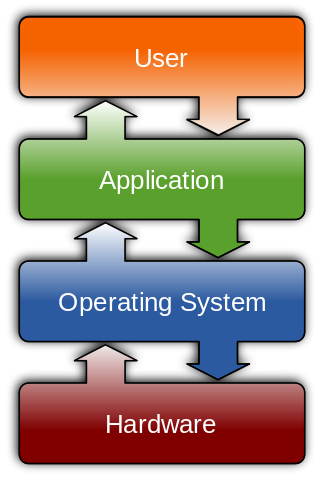
\includegraphics[height=2.5in]{OS/placement.png}

\end{minipage}
\begin{minipage}{4in}

\vspace{4pt}
\ans{Employee, Friend, Student, Teacher}

\vspace{32pt}
\ans{Chrome, Finder, PowerPoint, Word}

\vspace{32pt}
\ans{Android, Linux, Mac OS, Windows}

\vspace{32pt}
\ans{Desktop, Laptop, Phone, Tablet}

\end{minipage}


\quest{10 min}


\Q Consider a smartphone or tablet. Describe how users interact with applications.

\begin{answer}[5em]
Users interact by touching the screen, speaking out load, shaking the device, etc.
Apps respond by displaying results, playing sounds, sending notifications, etc.
\end{answer}


\Q With respect to hardware interactions, what does the operating system need to do?

\begin{answer}[5em]
The OS keeps track of resources; for example, it displays the battery life and clock time.
It also needs to coordinate all the apps that are currently running and manage the disk.
\end{answer}


\Q Why do applications need to go through the operating system to access hardware?

\begin{answer}[5em]
Having an OS between applications and hardware makes it easier to write software.
You don't have to worry about the details of all the devices (or lack thereof).
It also helps make the system more secure by not allowing programs to take over the machine.
\end{answer}
